\documentclass[11pt]{article}
\usepackage[margin=1in]{geometry}
\usepackage{amsmath}
\usepackage{graphicx}

\begin{document}

\title{Drying Algorithm}
%\author{Alex Griessman}
\date{\today}
\maketitle

\section{Composition}
Isotherms: $f(composition, temperature)$ (p.620 Table 10.2)

GAB Equation:
\[ \frac{M}{M_1} = \frac{K C a_w}{(1-C a_w)(1 + K C a_w - C a_w)} \]
\begin{align*}
\text{where: }& K_i = K_{o,i} e^{\Delta H_k/RT}\\
&C_i = C_{o,i} E^{\Delta H_c/RT}\\
&K = \sum_i K_i x_i\\
&C = \sum_i C_i x_i\\
\end{align*}

\section{Binding Energy}
p.612\\
Table 10-3 p.626

\begin{align*}
E_b = R\left(\frac{\partial\ln a_w}{\partial\left(\frac{1}{T}\right)_M}\right) \rightarrow &\ln\frac{a_{w1}}{a_{w2}} = \frac{E_b}{R}\left(\frac{1}{T_1}-\frac{1}{T_2}\right)_M \\
& \ln\frac{a_{w1}}{a_{w2}} = \frac{V_L}{RT}(P_2-P_1) \\
\end{align*}

\begin{center}
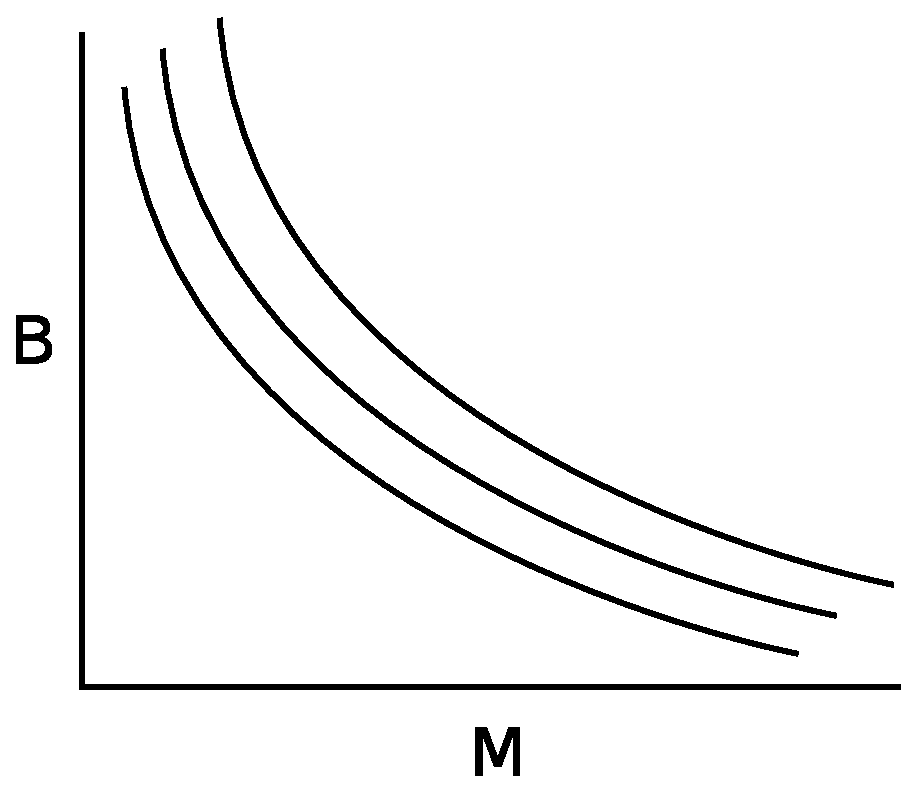
\includegraphics[width=0.4\textwidth]{pics/eps/binding_energy_1}
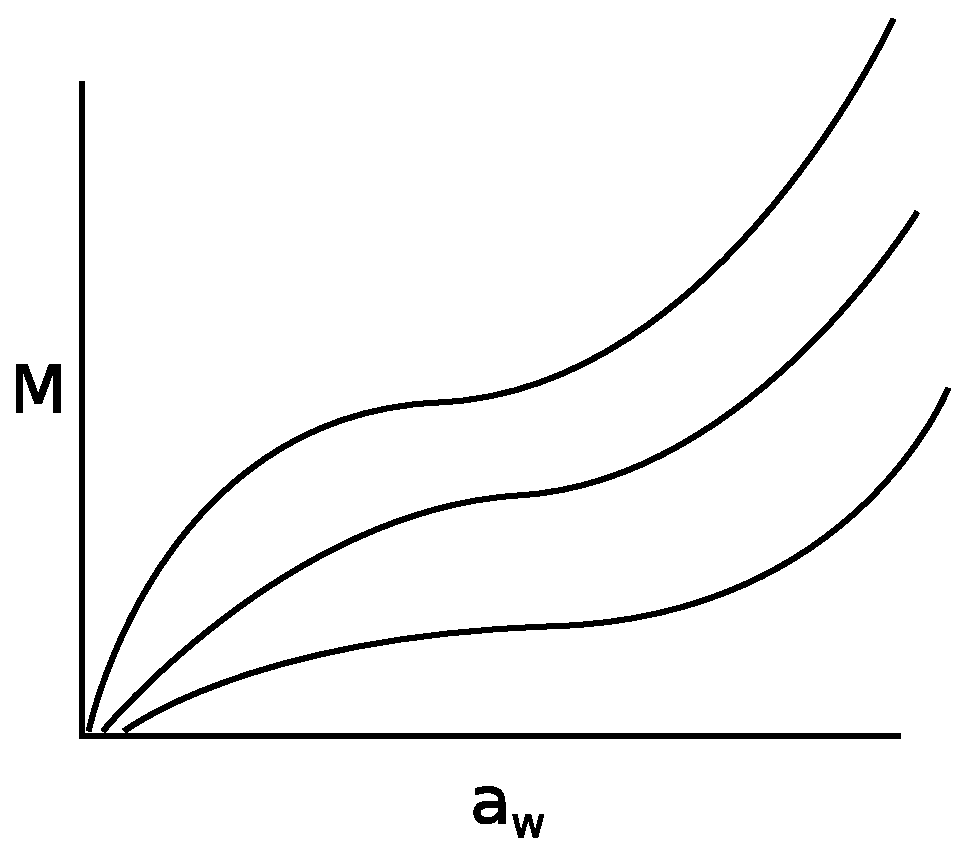
\includegraphics[width=0.4\textwidth]{pics/eps/binding_energy_2}
\end{center}

\section{Glass Transition}
Gordon Taylor: (Table 10.4 p.636)
\[ T_g = \frac{w_1 T_{g1} + K_2 w_2 T_{g2}}{w_1 + K_2 w_2} \]
\[ T_g = T_{g\infty} - \frac{K}{MW} \]

\begin{center}
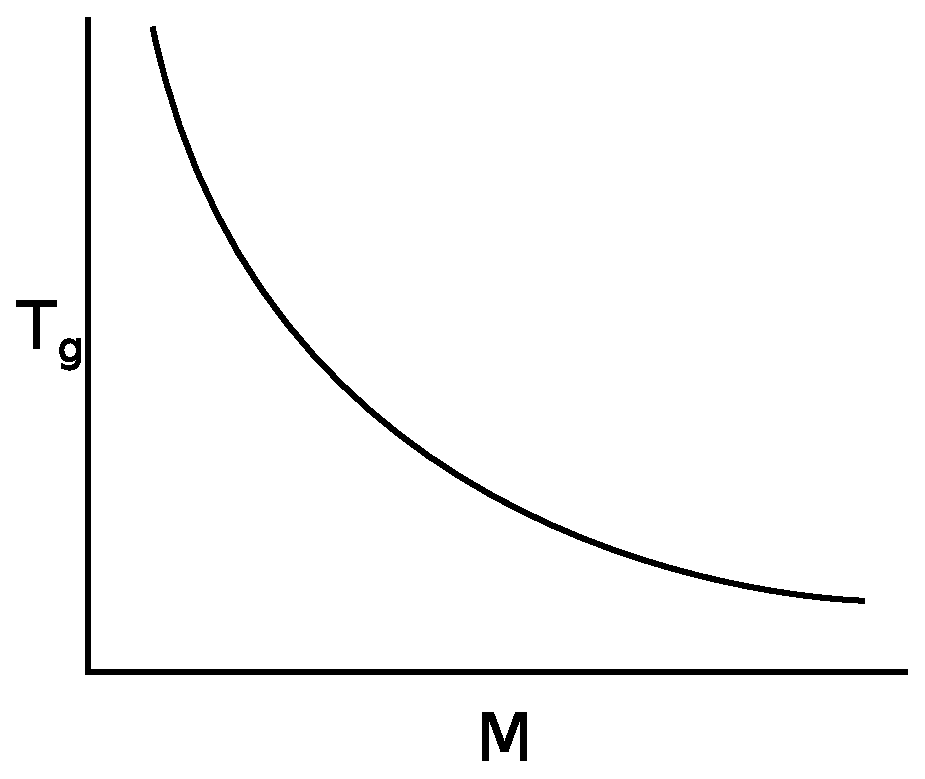
\includegraphics[width=0.3\textwidth]{pics/eps/glass_transition}
\end{center}

Williams-Landel-Ferry (WLF) Equation: (p.139 Lund)
\[ \ln\left(\frac{n}{n_g}\right) = \frac{-C_1 (T - T_g)}{C_2 + (T - T_g)} \]
\begin{align*}
\text{where: } &n_g = 10^{12} Pa \cdot s \\
& C_1 = 17.44\\
& C_2 = 5.16\\
\end{align*}

\section{Diffusivity}
Finite difference (p.506 Geankoplis)
\[ \frac{\partial M}{\partial t} = D_{eff} \frac{\partial^2 M}{\partial x^2} \]
Table 10-5 p.646
\[ D_{eff} \approx 10^{-9} - 10^{-12} \frac{m^2}{sec} \]
\[ D_{AVeff} = \frac{\epsilon}{\tau} D_{AV} = \frac{\epsilon}{\tau}(D_{AVD} e^{-E_c/RT}) \]
\[ D_{ALeff} = \frac{1-\epsilon}{\tau} D_{AL} = \frac{1-\epsilon}{\tau}(D_{ALD} e^{-E_A/RT}) \]
\[ D_{eff} = D_o e^{-E_a/RT} \]
\begin{align*}
\text{where: } & D_o = 6.39 \times 10^{-8} \frac{m^2}{s} \text{ (liquid)}\\
& D_o = 2.00 \times 10^{-5} \frac{m^2}{s} \text{ (gas)} \\
& E_a = 5.2 \frac{cal}{mol}\\
\end{align*}
$D_o$ depends on pore structure\\
H$_2$O Vapor: $2\times 10^{-5} m^2/s$\\
H$_2$O Liquid: $1\times 10^{-9} m^2/s$

\[ \frac{dF}{dt} = k_1(B) - k_2(F) = k_{10} e^{-E_1/RT}(B) - k_{20} e^{-E_2/RT}(F) \]
\[ \frac{dF}{dt} = 0 = \frac{F}{B} = \frac{k_{10}}{k_{20}} e^{(-E_1 + E_2)/RT} = Ke^{-E_b/RT} \]
\[ \frac{F}{F+B} = \frac{Ke^{E_b/RT}}{1+Ke^{-E_b/RT}} \rightarrow
\frac{D_{eff}}{D_o} = e^{-E_a/RT}\left(\frac{Ke^{-E_b/RT}}{1+Ke^{-E_b/RT}}\right) \]

\section{Porosity}
\subsection{Series}
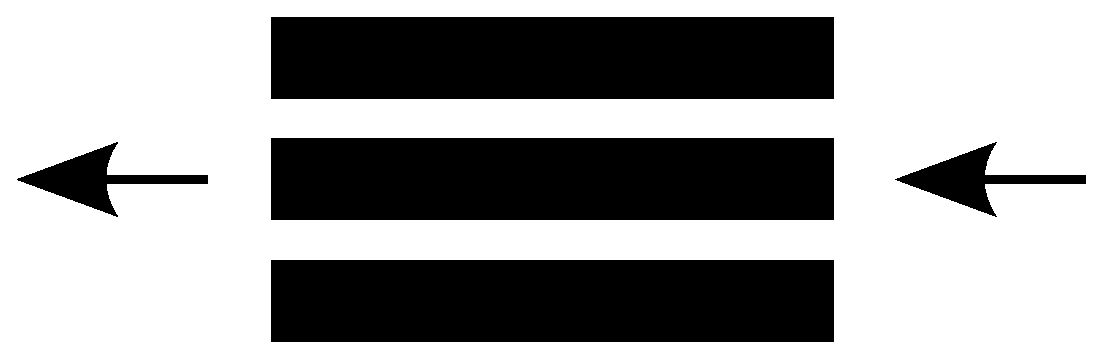
\includegraphics[width=0.3\textwidth]{pics/eps/porosity_series}
\[ D_{eff} = \frac{\epsilon}{\tau} D_v + \frac{1-\epsilon}{\tau} D_L \]
\subsection{Perpendicular}
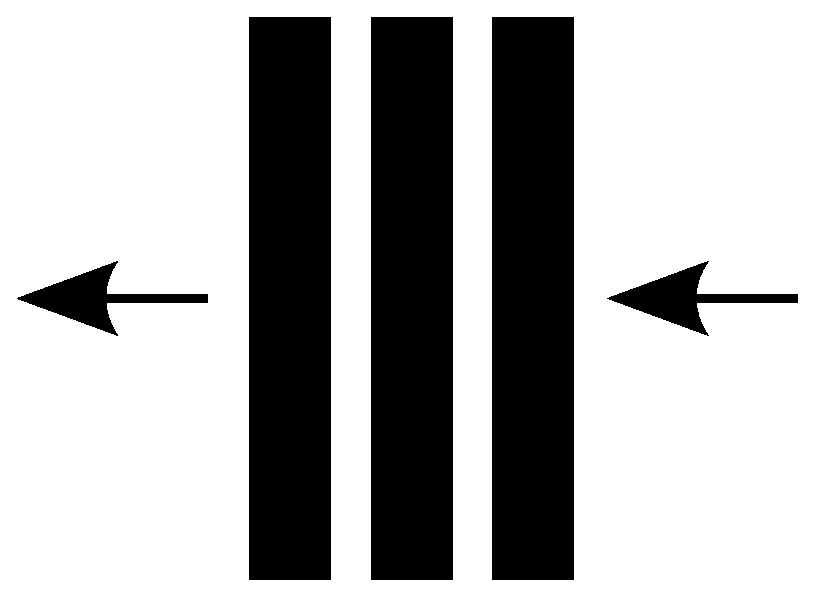
\includegraphics[width=0.3\textwidth]{pics/eps/porosity_perpendicular}
\[ \frac{1}{D_{eff}} = \frac{1}{\frac{\epsilon}{\tau}D_V} + \frac{1}{\frac{1-\epsilon}{\tau} D_L} \]

\subsection{Effective Diffusivity}
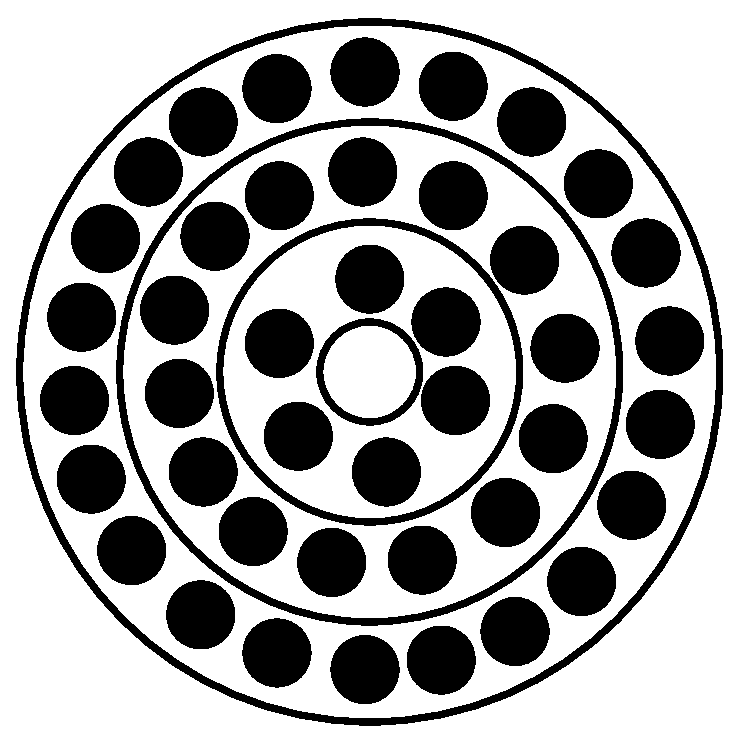
\includegraphics[width=0.3\textwidth]{pics/eps/porosity_circular}

\[ D_{AVeff} = \frac{\epsilon}{\tau} D_{AV} = \frac{\epsilon}{\tau} (D_{AVO}e^{-E_a/RT}) \frac{Ke^{-E_b/RT}}{1+Ke^{-E_b/RT}} \]
\[ D_{ALeff} = \frac{1-\epsilon}{\tau} D_{AL} = \frac{1-\epsilon}{\tau} (D_{ALO} e^{-E_a/RT}) \frac{Ke^{E_b/RT}}{1+Ke^{E_b/RT}} \]
\[ D_{eff} = \phi D_{eff=} + (1-\phi) D_{eff\bot} \]

\end{document}

